\documentclass[12pt,a4paper]{article}
\usepackage[utf8]{inputenc}

\usepackage{a4wide}

\newcommand{\FIMUreport}[5]{%
{
% Page layout -- do not change!!!
\renewcommand{\baselinestretch}{1.24}
\addtolength{\textheight}{2cm}
\addtolength{\topmargin}{-1cm}
\thispagestyle{empty}

\renewcommand{\familydefault}{ppl}
\renewcommand{\encodingdefault}{T1}
\renewcommand{\bfdefault}{bx}

\font \fntfilogo=fi-logo at 3.5cm
\newcommand{\fntfimu}{\fontencoding{T1}\fontfamily{ppl}\fontseries{m}%
     \fontsize{3.5cm}{3.5cm}\selectfont}
\newcommand{\fntstandard}{\fontencoding{T1}\fontfamily{ppl}\fontseries{b}%
     \fontsize{15pt}{17pt}\selectfont}
\newcommand{\fnttitle}{\fontencoding{T1}\fontfamily{ppl}\fontseries{b}%
     \fontsize{23pt}{25pt}\selectfont}
\fntstandard

\noindent
\raisebox{6ex}{\fntfilogo SL}
\hfill
{\fntfimu FI MU}\\[1ex]
\rule[1mm]{1.0\textwidth}{1.2pt}
\begin{flushright}
{\fntstandard Faculty of Informatics\\[.3ex] Masaryk University Brno}
\end{flushright}
\centering
\vfill

\begin{parbox}{\textwidth}{\centering\fnttitle #1}\end{parbox}
\vspace*{1.2cm}

by
\vspace*{1.2cm}

#2
\vfill

FI MU Report Series \hfill  FIMU-RS-#3-#5\\
\raisebox{1ex}{\rule{1.0\textwidth}{1.2pt}}
\raisebox{1ex}{Copyright  
\textcopyright{} #3, FI MU} \hfill
\raisebox{1ex}{#4\ #3}
\newpage
\thispagestyle{empty}
\newlength{\odsaz}
\settowidth{\odsaz}{Copyright \textcopyright{} #3,}
\noindent
\begin{tabbing}
Copyright
\textcopyright{} #3,\ \= Faculty of Informatics, Masaryk University.\\
\> All rights reserved. \\[1\baselineskip]
\> Reproduction of all or part of this work\\
\> is permitted for educational or research use\\
\> on condition that this copyright notice is\\
\> included in any copy. \\
\end{tabbing}
\vfill

\noindent
\begin{tabbing}
Publications in the FI MU Report Series are in general accessible \\via
WWW: \\[1ex]
\hspace{\odsaz}\ \= {\tt http://www.fi.muni.cz/reports/}\\[4ex]
%
Further information can be obtained by contacting: \\[1ex]
\> Faculty of Informatics\\
\> Masaryk University\\
\> Botanická 68a\\
\> 602\,00 Brno\\
\> Czech Republic
\end{tabbing}
}}


% Set up the base form.
\usepackage[resetfonts]{cmap} %% We need to load the T2A font encoding
\usepackage[T1,T2A]{fontenc}  %% to use the Cyrillic fonts with Russian texts.
\usepackage[
  main=english, %% By using `czech` or `slovak` as the main locale
                %% instead of `english`, you can typeset the thesis
                %% in either Czech or Slovak, respectively.
  czech         %% The additional keys allow
]{babel}        %% foreign texts to be typeset as follows:
\usepackage{geometry}
\usepackage[all]{nowidow}
\usepackage[protrusion]{microtype}
\makeatletter
\def\vnstyle{%
  \newgeometry{top=30mm,bottom=50mm,left=41mm,right=41mm,includeheadfoot}
  \renewcommand\section{\@startsection{section}{1}{\z@}%
                         {-15  \p@ \@plus -3\p@ \@minus -3\p@}%
                         {4\p@ \@plus 2\p@ \@minus 2\p@}%
                         {\normalfont\large\bfseries\boldmath
                          \rightskip=\z@ \@plus 8em\pretolerance=10000 }}
  \renewcommand\subsection{\@startsection{subsection}{2}{\z@}%
                         {-12\p@ \@plus -3\p@ \@minus -3\p@}%
                         {3\p@ \@plus 1\p@ \@minus 1\p@}%
                         {\normalfont\normalsize\bfseries\boldmath
                          \rightskip=\z@ \@plus 8em\pretolerance=10000 }}
  % \renewcommand\subsubsection{\@startsection{subsubsection}{3}{\z@}%
  %                        {-18\p@ \@plus -4\p@ \@minus -4\p@}%
  %                        {-0.5em \@plus -0.22em \@minus -0.1em}%
  %                        {\normalfont\normalsize\bfseries\boldmath}}
  % typesetting optimizations/setup
  \widowpenalty10000	% no windows
  \hfuzz2pt           % not to be bothered by \Overfulls of this size
  \abovedisplayskip =.3\abovedisplayskip
  \belowdisplayskip =.3\belowdisplayskip
  \setlength\intextsep{0pt}
  \abovecaptionskip =.5\abovecaptionskip
  \belowcaptionskip =.5\belowcaptionskip
  %\floatsep =.5\floatsep
  % Alter some LaTeX defaults for better treatment of figures:
      % See p.105 of "TeX Unbound" for suggested values.
      % See pp. 199-200 of Lamport's "LaTeX" book for details.
      %   General parameters, for ALL pages:
      \renewcommand{\topfraction}{0.9}	% max fraction of floats at top
      \renewcommand{\bottomfraction}{0.8}	% max fraction of floats at bottom
      %   Parameters for TEXT pages (not float pages):
      \setcounter{topnumber}{2}
      \setcounter{bottomnumber}{2}
      \setcounter{totalnumber}{4}     % 2 may work better
  %    \setcounter{dbltopnumber}{2}    % for 2-column pages
  %    \renewcommand{\dbltopfraction}{0.9}	% fit big float above 2-col. text
      \renewcommand{\textfraction}{0.07}	% allow minimal text w. figs
      %   Parameters for FLOAT pages (not text pages):
      \renewcommand{\floatpagefraction}{0.7}	% require fuller float pages
    % N.B.: floatpagefraction MUST be less than topfraction !!
  %    \renewcommand{\dblfloatpagefraction}{0.7}	% require fuller float pages
  }
\makeatother

% Additional paper-specific packages
\usepackage[colorlinks=true]{hyperref}
\usepackage[proportional,osf]{newpxtext}
\usepackage{mathpazo}
\usepackage[T1]{fontenc}
\usepackage{amsmath,amssymb}
\usepackage{array}
\usepackage{tikz}
\usetikzlibrary{positioning,fit,shapes,arrows}
\usepackage{booktabs}
\usepackage{xparse}
\usepackage{xspace}
\usepackage{rotating}
\usepackage{placeins}
\usepackage{floatpag}
\usepackage{bm}
\rotfloatpagestyle{plain}
\usepackage[
backend=biber,
style=iso-numeric,
sorting=none,
autolang=other,
sortlocale=auto,
maxcitenames=2,
]{biblatex}
\addbibresource{main.bib}
\addbibresource{sojka.bib}

% Additional paper-specific markup
\newcommand{\orcid}[1]{\href{https://orcid.org/#1}{\texttt{#1}}}
\newcommand{\email}[1]{\href{mailto:#1}{\texttt{#1}}}
\def\abbr#1{\textsc{\MakeLowercase{#1}}}
\newenvironment{liningfigs}{\renewcommand*{\rmdefault}{zpltlf}\normalfont}{}
\newif\ifthesis\thesisfalse
\newif\ifdebug\debugtrue
\newif\iflong\longtrue
\newif\ifreview\reviewfalse
\newcommand*\rot{\rotatebox{70}}
\newcommand{\op}[1]{\ensuremath{\operatorname{#1}}}
\newcommand{\avg}{\op{avg}}
\newcommand{\wavg}{\op{wavg}}
\newcommand{\sign}{\op{sign}}
\newcommand{\etal}{\unskip~\textit{et\penalty100\ al.}\xspace}
\newcommand{\longsubsection}[1]{\iflong\subsection{#1}\fi}
\def\abbr#1{\textsc{\MakeLowercase{#1}}}
\let\term\emph
\newcommand{\omid}{\rotatebox[origin=c]{-90}{$\ominus$}}
\makeatletter
\newcommand*{\bigominus}{\DOTSB\bigominus@\slimits@}
\newcommand{\bigominus@}{\mathop{\mathpalette\bigominus@@\relax}}
\newcommand{\bigominus@@}[2]{%
  \vcenter{\hbox{%
    \sbox\z@{$\m@th#1\bigoplus$}%
    \resizebox{\wd\z@}{!}{$\m@th#1\ominus$}%
  }}%
}
\makeatother
\newcommand{\bigomid}{\rotatebox[origin=c]{-90}{$\bigominus$}}
\NewDocumentCommand\todo{ggo}{%
  \ifdebug
    \textcolor{red}{TODO}%
    \IfValueT{#1}{\textcolor{red}{:~}}%
    \IfValueT{#1}{\textcolor{blue}{#1}}\nopagebreak%
    \IfValueT{#2}{\\\textcolor{orange}{#2}}\nopagebreak%
    \IfValueT{#3}{\\\textcolor{magenta}{#3}}%
  \fi}
% \done has the same args as \todo
\NewDocumentCommand\done{ggo}{%
  \ifdebug
    \textcolor{green}{DONE}%
    \IfValueT{#1}{\textcolor{green}{:~}}%
    \IfValueT{#1}{\textcolor{blue}{\sout{#1}}}\nopagebreak%
    \IfValueT{#2}{\\\textcolor{orange}{\sout{#2}}}\nopagebreak%
    \IfValueT{#3}{\\\textcolor{magenta}{\sout{#3}}}%
  \fi}
\newcommand*{\tran}{^{\mkern-1.5mu\mathsf{T}}}
\let\note=\footnote
\hyphenation{Wiki-pe-dia}
\let\emph=\textit
\let\subsubsection=\paragraph


% Every word in the title, except for short preposition and 
% connectives like, e.g., "in", "into", "for", "and", "or", etc.,
% should start with a capital letter.
\title{\bf Segmented Retrieval}

% First name(s) of each author should be written in full (e.g., "Frank Smith"
% instead of "F. Smith"). Accented letters must be specified by TeX 
% macros --- since the document is in English, do NOT use czech.sty and/or 
% CsLaTeX.
\author{%
  \textbf{Vít Novotný} and \textbf{Petr Sojka} \\
  Faculty of Informatics, Masaryk University \\
  Botanická 68a, 602\,00 Brno, Czechia \\
  \email{witiko@mail.muni.cz} and \email{sojka@fi.muni.cz} \\
  ORCID: \orcid{0000-0002-3303-4130} and \orcid{0000-0002-5768-4007}}
\date{November 8, 2017}

\hypersetup{%
unicode=true,
pdfencoding=auto,
pdftitle={Segmented Retrieval},
pdfauthor={Novotný, Vít; Sojka, Petr},
pdfkeywords={text retrieval; question answering; vector space modeling; text segmentation; semantic search; decay weighting},
}

\begin{document}

% The following command generates the cover page. The Year, Month, and nn
% (where nn is the report number) should be something like 2004, July, and 04,
% respectively. Remember that report numbers are assigned by the report 
% administrator. Also note that "\\" is not used after the name of the 
% last author.

\FIMUreport%
{Segmented Retrieval}%
{Vít Novotný \\ Petr Sojka}%
{2017}{November}{01}

% Now the front material is typeset. The page numbering is reset back to zero.
\setcounter{page}{0}
\vnstyle
\maketitle

% The abstract. The first line should NOT be indented. 
\begin{abstract}
\noindent
% elevator pitch
% struktura dle http://www.herout.net/blog/2013/12/jak-psat-abstrakt/:
%1) Jaký se řeší problém? Jaké je téma? Jaký je cíl textu?
%řeší se problém segmentace pro přesnější indexaci a vyhledávání 
%v textech.
Modern text retrieval systems employ text segmentation during the indexing of documents.
%2) Jak je problém vyřešen? Cíl naplněn?
%problém je řešen zpřesňováním sémantické reprezentace nugetů
%a vážením nugetů dle typu databáze (Godwin)
We show that, rather than returning the segments to the user,
significant improvements are achieved on the semantic text
similarity task by combining all segments % (nuggets)
from a single document into one result with an aggregate similarity score. 
%
%3) Jaké jsou konkrétní výsledky? Jak dobře je problém vyřešen?
%
%lépe než u SemEval 2016 a 2017
Following an analysis of the SemEval-2016 and 2017 task~3 datasets, we design a
segment decay weighting method that achieves state the art results on subtask~B
and can be readily implemented into existing inverted-index-based search
engines.
%4) Takže co? Čím je to užitečné Vědě a čtenáři?
% (Nebylo zde řečeno nic nového oproti bodu 2, takže jsem text zkrátil, čímž
% dostáváme k dobru řádek.)
% Ale ztracime tim udernou shrnujici vetu, ktera bude ve vsech indexacnich databazich
% typu WoS atp. Co tedy
% Segmentation in information retrieval matters, and leads to the best results in
% QA domain.
%
% Our results show that paying attention to important segments and using a
% task-specific weighting method leads to the best results on these question
% answering domain retrieval tasks.
%
%Take off: sémantická reprezentace dobře segmentovaných, tj. význam nesoucích částí je klíčem k úspěchu. důležité je i jejich vážení a agregace/výber dle specifik dokumentové sady a aplikace. 
\end{abstract}

\section{Introduction} 
%The vector space model (VSM)~\cite{ir:Salton1975} of representing documents,
%Representations of document semantics based solely on 
%document-term statistics, such as TF-IDF or 
%\href{https://en.wikipedia.org/wiki/Okapi_BM25}{Okapi BM25}, are 
%limited in their expressiveness and search precision.
%
%%Topics (topic modeling) of representing topic of documents
%
%Distributional semantics and deep learning allow building
%of semantic vector space models (SVSM) representing words, sentences,
%paragraphs or even whole documents as vectors in high-dimensional
%spaces~\cite{nlp:LSA1990,blei03lda,ml:mikolov2013distributed}.
%
%Segmentation matters: representation averaging over long
%documents chunks does not work: how to segment for indexing and search?
%
%Prior art, history of segmentation (token segmentation -> phrase segmentation (MI score Church, Hanks 1990
%-> sentence segmentation -> paragraph/semantic unit/thought/nugget segmentation)) 
%%%%%%%%%%%%%%%%%%%%%%%%%%%%
The standard bag-of-words vector space model~\cite{ir:Salton1975}\index{standard model|emph}
represents documents in terms of word % This is for ease of exposition, I use
% "term" and "token" in the rest of the document.
frequencies as vectors in high-dimensional real vector spaces.
\ifthesis The model disregards
word order, which immediately limits its ability to capture the meaning of a
document. Nevertheless, the \else The \fi model provides a notion of document
similarity that is well-understood and scales to large datasets. As a result,
it forms the basis of popular inverted-index-based search engines such as
Apache Lucene\index{Apache Lucene}~\cite{bialecki12}, and any improvements to
the model will have an immediate impact on the performance of a large body of
text retrieval applications.

Long documents that cover a range of different topics provide a significant
challenge for the standard model, since they are difficult to statically
summarize, and deemed irrelevant to most queries. For that reason,
we suggested~\cite{rygletal16}
to segment the indexed documents into semantically coherent
\term{nuggets}\index{nugget|emph}, and to retrieve these nuggets\index{nugget}
instead of the original documents. In \ifthesis this chapter\else the paper\fi,
we focus on the frequent
case, when the search engine is expected to retrieve full documents rather than
just the nuggets relevant to a query. It might seem that, in this scenario,
nuggets are useful for the summarization of results at best.  Contrary to this
intuition, we show that on our datasets, combining the evidence of similarity
provided by the retrieved nuggets yields significant improvements on the text
similarity task compared to standard model\index{standard model} on unsegmented
documents. Our results are fully reproducible.\note{%
\ifreview
A link to the research data will be disclosed in the camera-ready
version of the paper.
\else
\url{https://github.com/witiko-masters-thesis/segmentation}
\fi}

\ifthesis This chapter \else The paper \fi is structured as follows: In Section~\ref{sec:segmentation-relwork},
we review the related work. In Section~\ref{sec:segmentation-system}, we give an
overview of the system without delving into the specifics of our datasets. In
Section~\ref{sec:segmentation-experimental-setup}, we describe the parameter
estimation results, statistical observations, and techniques that we developed
specifically for our datasets.  Section~\ref{sec:segmentation-results} reports
the achieved results.  \iffalse 
In Section~\ref{sec:segmentation-qualitative-analysis},
we perform qualitative analysis of a small portion of our datasets to show the
effect of our methods compared to the standard model\index{standard model} on a
concrete example. 
\fi 
We conclude in Section~\ref{sec:segmentation-conclusion} by summarizing our results, and
suggesting future work.

%\section{Problem Formulation, Related Work and Experimental Setup}
%\label{setup}
%
% the playground and problem formulation
% \longsubsection{Problem Formulation}
%
% document representation as point in vector space 
% -> representation of document segments as points in vector space
%
% search as similarity computation between query and documents' segments
% -> 1) how to segment 2) how to represent segments 3) how to measure segment similarity
% 4) how to aggregate matrix of query and documents' segment similarity
% into final similarity ranking

% related work in 1), 2), 3) and 4) 
%\longsubsection{Related Work}

\section{Related work}
\label{sec:segmentation-relwork}
The notion of representing a document as a vector\index{standard model} of term
weights, and estimating the similarity between two documents by the cosine of
the angle between their vectors
was perhaps first explored by \textcite{ml:salton71smart} during his work on the
\abbr{SMART} information retrieval system. Several
competing methods for assigning term weights and normalizing document vectors
were proposed in literature. In this work, we consider those presented by
\textcite{ml:SaltonBuckley1988,singhaletal95,%or https://dl.acm.org/citation.cfm?id=243206
murataetal00}.

The probabilistic Okapi \abbr{BM}25\index{Okapi \abbr{BM}25} model is an alternative to Salton's vector space
model and was developed %at \abbr{TREC} 
by \textcite{robertsonetal76,\ifthesis robertsonetal94,\fi robertsonetal95}. In this work, we consider the version of the model
that \textcite{singhal01} describes as the state of the art.

Assessing the similarity of two structured documents by combining the evidence
of similarity provided by their \term{structural elements} (e.g.\
nuggets)\index{nugget} has already been explored in the context
of \abbr{XML}\index{XML@\abbr{XML}} document retrieval. In this work, we draw
inspiration from
\abbr{IBM} Haifa's Juru\abbr{XML} system described by \textcite{massetal02}.
However, whereas \abbr{XML} documents have a tree structure, which makes it
possible to compare segments on the basis of structural similarity, the system
described in this work makes no assumptions about the structure of nuggets.

Improving unstructured text retrieval by removing or assigning different
weights to \term{document zones} (e.g.\
nuggets)\index{nugget} has been of interest to researchers in the fields of
text summarization, feature selection, and text classification. In this work, I
consider the approaches of \textcite{kolczetal00,koetal04}.

% References to Raslan 2016 in
%
% 1) Related work in how to segment: 
% ... 
%
% 2) Related work in how to represent segments:
% different weighting schemes, BM25, ...
%
% 3) Related work in how to measure segment similarity:
%
% 4) Related work in how to aggregate matrix of query and documents' segment similarity
% into final similarity rankings: max pooling, averaging, segment weighting
%
% References to Raslan 2016 in above, experimental system architecture.
%
% Specifics of segmentation of different IR: 
% we have evaluated on Q/A task. 
%
% \motto Experts often possess more data than judgment. Colin Powell \\-2
% Read more at: http://www.brainyquote.com/quotes/keywords/data.html

\section{System description}
\label{sec:segmentation-system}
Our system takes as input a list of nuggets\index{nugget} that form a single document, and
preprocesses them. Given a preprocessed query document and a preprocessed
result document, our system computes a single aggregate score that captures the
similarity between the two documents.
In the following subsections, we break the system into its individual components
and describe each one in detail.

% \section{Dataset, Data Preprocessing} % data
% Semeval 2016, 2017 task 3 \cite{nakov2017semeval}
%
% data preprocessing
%
% data analysis, outcomes from data analysis (Godwin)
%
% word and segment weighting 
% 
% \section{Methods and Methodology, Evaluation Metrics} % +algorithms 
% \label{methods}
% 
% List of all free variables/axes in 1--4) above (description of parameter's space
% with arguments why they might be relevant).
% 
% tokenisation pipeline, word representation and weighting
% 
% segments weighting 
% 
% pivoting
% 
% ... TODO
\subsection{Nugget filtering}\index{nugget!filtering|emph}
\label{sec:segmentation-nugget-filtering}
As a first preprocessing step, we take each nugget\index{nugget} and make a prediction about
its importance. If the predicted importance falls below a threshold, we remove
the nugget. Under the hypothesis that only important nuggets contain (with a
higher chance than random) important terms that describe the meaning of a
document, this step extracts a summary with a high density of important terms.

In this work, we consider the following text summarization techniques proposed
by \textcite{kolczetal00}, which we modify to use nuggets\index{nugget} rather than
sentences and paragraphs as the base unit of text:
\begin{description}
\item[Title\index{.title@Title|emph}] All nuggets\index{nugget} other than the nugget corresponding to the title of a
  text document (title nugget) are removed.
\item[FirstPara\index{.firstpara@FirstPara|emph}] All nuggets\index{nugget} other than the title nugget, and other than the
  first non-title nugget are removed.
\item[FirstTwoPara\index{.firsttwopara@FirstTwoPara|emph}] All nuggets\index{nugget} other than the title nugget, and other than the
  first two non-title nuggets are removed.
\item[FirstLastPara\index{.firstlastpara@FirstLastPara|emph}] All nuggets\index{nugget} other than the title nugget, the first
  non-title nugget, and the last non-title nugget are removed.
\item[ParaWithMostTitleWords\index{.parawithmosttitlewords@ParaWithMostTitleWords|emph}] All nuggets\index{nugget} other than the title nugget, and
  other than the first non-title nugget that contains the highest number of
  tokens present in the title nugget (title tokens) are removed.
\item[BestSentence${}_l$\index{.bestsentence@BestSentence${}_l$|emph}] All nuggets\index{nugget} other than the title nugget, and other than
  the nuggets that contain less than $l$\index{.l@$l$|emph} title tokens are removed.
\end{description}
Note that the Title\index{.title@Title},
ParaWithMostTitleWords\index{.parawithmosttitlewords@ParaWithMostTitleWords},
and BestSentence${}_l$\index{.bestsentence@BestSentence${}_l$} techniques
assume that a document contains a title, subject, abstract, or other form of a
short summary. These techniques cannot be used without modification if this
assumption is violated.

\subsection{Scoring function}
\label{sec:segmentation-scoring-function}
\subsubsection{Indexing}
If we are indexing the nuggets\index{nugget}, then for each nugget $i$ that was not removed
in the previous step, we record in the inverted index the term frequency vector
$\mathbf{f}_i$\index{.fi@$\mathbf  {f}_i$|emph}, where $f_{it}$ is the frequency of
term $t$ in nugget $i$,
the number of tokens $\sum_t f_{it}$ in nugget $i$, and the vector
$\mathbf{p}_i$, where $p_{it}$ is the location where term $t$ first occures in
the document that contains nugget $i$.

We also update the collection-wide statistics that consist of the total number
of nuggets\index{nugget} in the collection~$N$\index{.n@$N$|emph} (collection size), the number of nuggets~$n_t$
that contain term~$t$ (nugget frequency), the average nugget length
$\avg_i(\sum_t f_{it})$, the average number of terms in a nugget $\avg_i u_i$\index{.ui@$u_i$|emph},
and the average byte length of a nugget $\avg_i b_i$\index{.bi@$b_i$|emph}.

\subsubsection{Querying}
If the nuggets\index{nugget} come from a query document, then for each nugget~$i$ that was
not removed in the previous step, we traverse the inverted index, searching
for candidate nuggets~$j$ that have at least one term in common with nugget~$i$.
For every $i,j$, we compute the similarity score $S(i, j)$\index{.s@$S$|emph}.

With the standard model\index{standard model}~\cite{ir:Salton1975}, we first
map the nuggets\index{nugget} $i,j$ to
nugget vectors $\mathbf{v}_i,\mathbf{v}_j$. The formulas for the vectors
depend on our weighting scheme. A~naming convention for the various weighting
schemes was proposed by \textcite{ml:salton71smart} during his work on the \abbr{SMART}
information retrieval system and further extended in
subsequent research~\cite{ml:SaltonBuckley1988,singhaletal95} (see
Table~\ref{tab:segmentation-smart}).  Using this convention, every weighting scheme can be
assigned a name in the form of
$\mathbf{t}_j\mathbf{d}_jm_j$\texttt{.}$\mathbf{t}_i\mathbf{d}_im_i$, where
$\mathbf{t}_c, \mathbf{d}_c$, and $m_c, c=i,j,$ stand for the term frequency,
nugget frequency, and nugget length normalization factors, respectively.
The nugget vectors $\mathbf{v}_c$ then equal
$\mathbf{t}_c\circ\mathbf{d}_cm_c^{-1}$, where $\circ$ denotes the entrywise
(Hadamard) product. E.g. if we choose \texttt{bfx.nfx} as our weighting scheme,
then $\mathbf{v}_j=\sign(\mathbf{f}_j)\circ\ln\frac{N}{\mathbf
n},\mathbf{v}_i=\mathbf{f}_i\circ\ln\frac{N}{\mathbf n}$.

We also consider the term weighting method described by Murata et
al.~\cite{murataetal00}, which we will refer to as the
\term{Murata} weighting method. The weight
$K_{\textrm{location}}(i, t)$ of term~$t$ in a nugget\index{nugget} $i$
penalizes terms that appear near the end of a nugget and is defined as follows:
\begin{equation*}
  K_{\textrm{location}}(i, t) = \begin{cases}
    k_{\textrm{location},1} & \text{if $t$ occurs in a title nugget,} \\
    1 + k_{\textrm{location},2}\frac{\sum_t f_{it}-2p_{it}}{\sum_t f_{it}} & \text{otherwise,}
  \end{cases}
\end{equation*}
where $k_{\textrm{location},1}$, and $k_{\textrm{location},2}$ are
parameters that the authors set to $k_{\textrm{location},1}=1.35$, and
$k_{\textrm{location},2}=0.125$ in their system A (we will refer to this
method as Murata$_{\textrm A}$\index{.murataa@Murata$_{\textrm A}$|emph} for ease
of reference), and to
$k_{\textrm{location},1}=1.3$, and $k_{\textrm{location},2}=0.15$ in their
system B (we will refer to this method as Murata$_{\textrm
B}$\index{.muratab@Murata$_{\textrm B}$|emph} for ease of reference). If we let
$\mathbf{e}$\index{.e@$\mathbf{e}$|emph} denote the supplementary weight
vector, such that $e_t = K_{\textrm{location}}(i, t)$. Then
$\mathbf{v}_c=\mathbf{t}_c\circ\mathbf{e}\circ\mathbf{d}_cm_c^{-1}$, where
the vector length normalization factor $m_c$ corrects for the final weights
$\mathbf{w}_c=\mathbf{t}_c\circ\mathbf{e}\circ\mathbf{d}_c$. Additional
choices of the supplementary weight vector $\mathbf{e}$\index{.e@$\mathbf{e}$}
were considered as a part of the dataset analysis in
Section~\ref{sec:segmentation-dataset-analysis}.

Regardless of whether or not we use the supplementary weight vector
$\mathbf{e}$\index{.e@$\mathbf{e}$}, the value of the scoring function $S(i,
j)$\index{.s@$S$} equals $\mathbf v_i\tran \mathbf v_j$ in the standard
model\index{standard model}.

\begin{table}[tb]
\centering
\begin{tabular}{>{\ttfamily}rl>{\ttfamily}rl>{\ttfamily}rl}
\multicolumn{2}{c}{Term frequency} &
  \multicolumn{2}{c}{Nugget frequency} &
  \multicolumn{2}{c}{Normalization} \\ \toprule
b & $\sign(\mathbf{f}_{i})$ &
  x\textrm{, }n & $\mathbf{1}$ &
  x\textrm{, }n\index{.n@\texttt{n}|emph} & 1 \\
t\textrm{, }n & $\mathbf{f}_{i}$ &
  f & $\mathbf{1}\cdot\ln\frac N{\mathbf{n}}$ &
  c & $\sqrt{\mathbf w_{i}\tran \mathbf w_{i}}$ \\
a & $\mathbf{0.5}+0.5\frac{\mathbf{f}_{i}}{\max_tf_{it}}$ &
  t\index{.t@\texttt{t}|emph}    & $\mathbf{1}\cdot\ln\frac{N+1}{\mathbf{n}}$ &
  u\index{.u@\texttt  {u}|emph}    & $1-s + s\frac{u_i}{\avg_iu_i}$ \\
l    & $\mathbf{1}+\ln \mathbf{f}_{i}$ &
  p    & $\mathbf{1}\cdot\ln\frac{N-n_t}{\mathbf{n}}$ &
  b\index{.b@\texttt  {b}|emph}    & $1-s + s\frac{b_i}{\avg_ib_i}$ \\
L    & $\frac{\mathbf1+\ln \mathbf{f}_{i}}{1+\ln(\avg_tf_{it})}$ & & & & \\
d    & $\mathbf1+\ln(\mathbf1+\ln \mathbf{f}_{i})$ & & & &\\
\end{tabular}
\caption[The \abbr{SMART} notation for the weighting schemes]{The \abbr{SMART}
  notation for the weighting schemes 
  used with the standard model\index{standard model}, where $f_{it}$ is the
  frequency of term~$t$ in a nugget\index{nugget}~$i$ (term frequency),
  $\mathbf{f}_i$\index{.fi@$\mathbf{f}_i$} is the vector of term frequencies in
  a nugget~$i$, $N$\index{.n@$N$}~is the total number of nuggets in the
  collection (collection size), $n_t$ is the number of nuggets
  that contain term $t$ (nugget frequency), $\mathbf{n}$\index{.n@$\mathbf{n}$}
  is the vector of nugget frequencies, $u_i$\index{.ui@$u_i$}
  is the number of terms in a nugget $i$, $b_i$\index{.bi@$b_i$} is the byte length of nugget
  $i$, $\mathbf{w}_{i}$ is the vector of term weights in a nugget~$i$, and
  $s$\index{.s@$s$|emph} is the slope in the context of pivoted document length
  normalization.  Letters on the left uniquely identify each term frequency,
  nugget frequency, and nugget length normalization factor.}
\label{tab:segmentation-smart}
\end{table}

If instead of the standard model\index{standard model} we use the Okapi
\abbr{BM}25 model\index{Okapi \abbr{BM}25|emph}, then we define the scoring
function $S(i,j)$\index{.s@$S$} as follows~\cite{singhal01}:
\begin{equation*}
  \textstyle
  S(i,j) = \sum_{\textrm{term }t\in i,j}
  \ln\frac{N-n_k+0.5}{n_k+0.5}\cdot
  \frac{(k_1+1)f_{jt}}{k_1\left((1-b)+b\frac{\sum_t
  f_{jt}}{\avg_i(\sum_t f_{it})}\right)+f_{jt}}\cdot\frac{(k_3+1)f_{it}}{k_3+f_{it}},
\end{equation*}
where $k_1\in[1,2], k_3\in[0,1000],$ and $b\in[0,1]$ are parameters.%
\index{.k1@$k_1$|emph}\index{.k3@$k_3$|emph}\index{.b@$b$|emph}

\subsection{Result aggregation}
\label{sec:segmentation-result-aggregation}
If we are indexing a document, then the previous two steps (filtering and
scoring) conclude our efforts. If, instead of indexing a document, we are
processing a query document~$u$, then we have just retrieved a number of
candidate nuggets\index{nugget} that are highly similar to at least one of the query nuggets
according to our scoring function~$S$\index{.s@$S$}. Our task now is to use this information
to return documents that satisfy the user's information need.

\subsubsection{Unsegmented approach}
If we performed no segmentation, then a nugget\index{nugget} corresponds directly to a
document. In this scenario, we return to the user each candidate nugget $j$ in
decreasing order relative to the scoring function $S(i, j)$\index{.s@$S$}, where $i$ is the
single unsegmented query nugget.

If we performed segmentation, then for each document $v$ (result document)
having at least one nugget\index{nugget} in the set of candidate nuggets, we retrieve the full
set of $v$'s nuggets (result nuggets) and we compute a similarity matrix
$\mathbf{M}_{uv}$\index{.muv@$\mathbf  {M}_{uv}$|emph}, where every row contains the scores between a single query
nugget from $u$ and all result nuggets from $v$ and every column contains the
scores between all query nuggets from $u$ and a single result nugget from~$v$.
We are now interested in finding an aggregate scoring function $S'(u, v)$\index{.s'@$S'$|emph} that
is expressed in terms of the elements of $\mathbf{M}_{uv}$\index{.muv@$\mathbf  {M}_{uv}$}\ifthesis, such that
the ordering of result documents induced by $S'$\index{.s'@$S'$} correlates with the relevance
of the result documents $v$ to the information need behind the query document
$u$\fi.

Should there be no upper bound on the number of nuggets\index{nugget} in query and result
documents, then the computation of $\mathbf{M}_{uv}$\index{.muv@$\mathbf  {M}_{uv}$}
may turn out to be prohibitively slow. One possible approach to speeding up the
retrieval is to forgo the segmentation of query documents and to segment only
the result documents instead.  This is the standard approach in semi-structured
\abbr{XML} retrieval~\cite{massetal02}, where the query constitutes only a
single branch of an \abbr{XML}\index{XML@\abbr{XML}} document tree. In our
experiments, we did not evaluate this approach.

\subsubsection{Machine learning approach}
It may happen that the indexed documents share the same structure, and the
segmentation is predictable in that it always produces the same number of
nuggets\index{nugget} both per a query document and per a result document. If there is also
annotated training data available, then we can build a classifier beforehand
using the following procedure. For each query document~$u$, result document~$v$,
and the corresponding relevance judgement, we concatenate the rows of
$\mathbf{M}_{uv}$\index{.muv@$\mathbf  {M}_{uv}$} into a feature vector
$\mathbf{x}_{uv}$\index{.xuv@$\mathbf x_{uv}$|emph}. We then perform logistic
regression on the list of feature vectors and the corresponding relevance
judgements to fit a classifier that assigns a posterior probability estimate
$\hat P(\textrm{relevant}\mid\mathbf{x}_{uv})$ to any $u$ and~$v$.  Our desired
aggregate scoring function is then $S'(u, v) = \hat
P(\textrm{relevant}\mid\mathbf{x}_{uv})$\index{.s'@$S'$}.

In practice, the segmentation is likely to produce a variable number of nuggets\index{nugget}
per document. In that scenario, we can treat matrix
$\mathbf{M}_{uv}$\index{.muv@$\mathbf  {M}_{uv}$} as a greyscale image
$\mathbf{I}_{uv}$\index{.iuv@$\mathbf  {I}_{uv}$|emph} (see
Figure~\ref{fig:segmentation-computing-muv}), and set
$S'(u, v)=\hat P(\textrm{relevant}\mid\mathbf{I}_{uv})$, where $\hat
P(\textrm{relevant}\mid\mathbf{I}_{uv})$ is the posterior probability of an
image classifier. In our experiments, we did not evaluate this approach.

\begin{figure}[t]
\begin{center}
\scriptsize
\tikzset{nugget/.style={draw, text width=2cm}}
\begin{tikzpicture}[baseline=(current bounding box.center)]
\node (1) [nugget]                 {$u_1$: I did enact Julius \textbf{Caesar}};
\node (2) [nugget,below=.1cm of 1] {$u_2$: I \textbf{was} killed i' \textbf{the} Capitol};
\node (3) [nugget,below=.1cm of 2] {$u_3$: \textbf{Brutus} killed me};

\node (A) [nugget,right=.5cm of 1] {$v_1$: So let it be with \textbf{Caesar}};
\node (B) [nugget,below=.1cm of A] {$v_2$: \textbf{The} noble \textbf{Brutus} hath told you};
\node (C) [nugget,below=.1cm of B] {$v_3$: \textbf{Caesar was} ambitious};

\draw[-, line width=0.09128709291752768557em, draw=white!18.257418583505537114!black] (1.east) to (A.west);
\draw[-, line width=0.12909944487358056283em, draw=white!25.819888974716112567!black] (1.east) to (C.west);
\draw[-, line width=0.08333333333333333333em, draw=white!16.666666666666666666!black] (2.east) to (B.west);
\draw[-, line width=0.11785113019775792073em, draw=white!23.57022603955158414600!black] (2.east) to (C.west);
\draw[-, line width=0.11785113019775792073em, draw=white!23.57022603955158414600!black] (3.east) to (B.west);
\end{tikzpicture}%
{\begin{minipage}{4.1cm}
${}\leadsto\mathbf{M}_{uv} = \left(\begin{matrix}
  0.18 & 0    & 0.26 \\
  0    & 0.16 & 0.24 \\
  0    & 0.24 & 0    \\
\end{matrix}\right)$
\end{minipage}{%
\begin{minipage}{2.6cm}\vspace*{1.2ex}
$\textstyle\raisebox{-.5ex}{\rotatebox[origin=c]{10}{$\leadsto$}}\ \bigomid_i\bigominus_j m_{ij} = 0.205 \\[.5em]
\raisebox{.5ex}{\rotatebox[origin=c]{-10}{$\leadsto$}}\ \mathbf{I}_{uv} = 
\begin{tikzpicture}[baseline={([yshift=-.8ex]current bounding box.center)}, scale=0.3]
  \def\pixels{
    {2,0,4},
    {0,1,3},
    {0,3,0},
  }
  \definecolor{pixel 0}{HTML}{FFFFFF}
  \definecolor{pixel 1}{HTML}{D6D6D6}
  \definecolor{pixel 2}{HTML}{D1D1D1}
  \definecolor{pixel 3}{HTML}{C2C2C2}
  \definecolor{pixel 4}{HTML}{BDBDBD}
  \foreach \line [count=\y] in \pixels {
    \foreach \pix [count=\x] in \line {
      \draw[fill=pixel \pix] (\x,-\y) rectangle +(1,1);
    }
  }
\end{tikzpicture}$
\end{minipage}}}
\end{center}
\caption[Using the handcrafted operators]{%
  Given query and result documents $u$ and $v$ consisting of
  nuggets\index{nugget} $u_1,u_2,u_3,v_1,v_2,$ and $v_3$, we compute a similarity
  matrix $\mathbf{M}_{uv}$\index{.muv@$\mathbf{M}_{uv}$} using the
  \texttt{bnc.bnc} standard model weighting scheme. Using the handcrafted
  operators
  $\ominus=\protect\omid=\wavg_{\textrm{length}}$\index{.ominus@$\ominus$}\index{.omid@$\kern.2ex\protect\omid$}\index{.wavglength@$\protect\wavg_{\textrm{length}}$},
  we compute the aggregate score $S'_{\text{result-first}}$%
  \index{.s'resultfirst@$S'_{\text{result-first}}$} (above), or we
  convert $\mathbf{M}_{uv}$ to a grayscale image
  $\mathbf{I}_{uv}$\index{.iuv@$\mathbf{I}_{uv}$} that we pass to an image
  classifier (below).}
  \label{fig:segmentation-computing-muv}
\end{figure}

\subsubsection{Hand-crafted operators}
Having apriori knowledge about our documents allows us to construct rules that
describe which query and result nuggets\index{nugget} will contribute the most to the
aggregate scoring function $S'$. Let
$\ominus,\omid$\index{.ominus@$\ominus $|emph}\index{.omid@$\kern .2ex\omid $|emph}
be associative and
commutative \ifthesis binary \fi operators \ifthesis on $\mathbb{R}$ \fi and let $m_{ij}$
denote the value of a matrix $\mathbf{M}_{uv}$\index{.muv@$\mathbf  {M}_{uv}$} in the row and column corresponding to the
query and result nuggets $i$ and~$j$. Then we can express our aggregate scoring
function as either
\begin{align*}
S'_{\textrm{query-first}}(u,v) &= \textstyle\bigominus_{\textrm{result nugget }j\in v}
  \bigomid_{\textrm{query nugget }i\in u} m_{ij}\text{, or}
  \index{.s'queryfirst@$S'_{\text  {query-first}}$|emph}\\
S'_{\textrm{result-first}}(u,v) &= \textstyle\bigomid_{\textrm{query nugget }i\in u}
  \bigominus_{\textrm{result nugget }j\in v} m_{ij}\text{ (see Figure~\ref{fig:segmentation-computing-muv})}.%
  \index{.s'resultfirst@$S'_{\text  {result-first}}$|emph}
\end{align*}
In our experiments, we evaluated $\ominus,\omid\in\{\min,\max,\avg,\wavg\}$%
\index{.ominus@$\ominus $}\index{.omid@$\kern .2ex\omid $}
with various weighting methods for the $\wavg$ operator, such as
$\wavg_{\textrm{length}}$\index{.wavglength@$\wavg _{\textrm  {length}}$|emph}, which assigns weights proportional to the
number of tokens in a nugget\index{nugget}, and $\wavg_{\textrm{Koetal}}$%
\index{.wavgKoetal@$\wavg_{\textrm{Koetal}}$|emph} inspired by the
work of \textcite{koetal04}, which assigns weights proportional to the
score between a nugget and the title nugget of its document. Additional
weighting methods were developed as a part of the dataset analysis (see
Section~\ref{sec:segmentation-dataset-analysis}). Note that for
$\ominus,\omid\in\{\avg,\wavg\},$ we obtain $S'_{\textrm{query-first}} =
S'_{\textrm{result-first}},$
\index{.s'queryfirst@$S'_{\text  {query-first}}$}
\index{.s'resultfirst@$S'_{\text  {result-first}}$}
and that for $\ominus,\omid\in\{\min,\max,\avg\}$ such that $\ominus=\omid$,
the following holds:
\begin{equation*}
  S'_{\textrm{query-first}}(u,v) = S'_{\textrm{result-first}}(u,v) =
  \textstyle\bigominus_{\textrm{result\,nugget\,}j\in
  v,\textrm{\,query\,nugget\,}i\in u} m_{ij}.
\end{equation*}

\section{Experimental setup}
\label{sec:segmentation-experimental-setup}
In our experiments, we evaluated the systems on the SemEval-2016 and 2017
task~3 subtask~B question answering (\abbr{QA})\index{qa@\abbr{QA}} datasets.
These datasets consist of discussion threads from the Qatar
Living\note{\url{http://www.qatarliving.com/forum}} internet forum. Given
an original question, and a set of ten candidate threads containing both a
related question and the initial ten comments in the thread, the task is to
rank the candidate threads by their relevance to the original
question.~\cite{preslavetal16,nakov2017semeval} The performance of a system
is evaluated by its mean average precision\index{map@\abbr {MAP}|emph}
(\abbr{MAP}) using relevance judgements.

The SemEval-2016 task~3 subtask~B datasets consist of the training dataset (267
original questions, 1,790~threads), the dev dataset (50~original questions,
244~unique threads), and the test dataset (70~original questions, 327~unique
threads). The winning SemEval-2016 task~3 subtask~B submission was
\term{\abbr{UH-PRHLT}-primary} with a \abbr{MAP}\index{map@\abbr {MAP}} score of
$76.7$. SemEval-2017 task~3 subtask~B uses the same training and dev datasets as
SemEval-2016 with the provision that the SemEval-2016 test dataset can be used
for training. A new test dataset (88 original questions, 293 unique threads)
has also been added.  The SemEval-2017 task~3 subtask~B winning configuration
was \term{SimBow-primary} with a \abbr{MAP}\index{map@\abbr {MAP}} score of $47.22$.

We also used the SemEval-2016 and 2017 task~3 subtask~A datasets for
statistical analysis. These datasets contain the same data (2,654 questions,
26,540 comments) as the subtask~B training datasets, but now the relevance
judgements assess how relevant a comment is to a question.  For language
modelling, the unannotated SemEval-2016 and 2017 task~3 subtask~A
datasets (189,941 questions, 1,894,456 comments) are available.

\subsection{Language modeling and segmentation}
\label{sec:segmentation-language-modeling-segmentation}
The texts in the datasets were lower-cased, stripped of images and \abbr{URL}s,
and tokenized on white spaces and punctuation. Tokens shorter than two
characters or longer than 15~characters were removed. Using the existing
structure of the datasets, every original question was split into two nuggets\index{nugget}
corresponding to the question subject and text, and every candidate thread was
split into twelve nuggets corresponding to the related question subject and
text, and the initial ten comments.

Since the annotated datasets did not contain enough text to build a proper
language model, we used the unannotated subtask~A datasets to obtain the
collection-wide statistics required to compute the scoring function described
in Section~\ref{sec:segmentation-scoring-function}.

\subsection{Dataset analysis}
\label{sec:segmentation-dataset-analysis}
In 1991, the American attorney and author Mike Godwin formulated%
\note{\url{news:1991Aug18.215029.19421@eff.org}} a rule that ``as a Usenet
discussion grows longer, the probability of a comparison involving Nazis or
Hitler approaches one.'' An immediate corollary would be that as an online
discussion grows longer, the probability of a relevant contribution approaches
zero. We were curious whether the datasets would confirm these observations.

We used the subtask~A relevance judgements to estimate the probability mass
function $\hat P(\textrm{at position }i\mid\textrm{relevant})$ for
$i=1,2,\ldots,10$. Since there is a uniform number of comments at each
position $i$, e.g. $\hat P(\textrm{at position }i) = 0.1$, we would expect
$\hat P(\textrm{at position }i\mid\textrm{relevant})$ to be also uniform if
the position of a comment and its relevance are independent.
Figure~\ref{fig:dataset-relevance-analysis} shows that this expectation is
false, and that there seems to be an inverse relationship between the position
of a comment and its relevance.

\begin{figure}[tb]
\centering
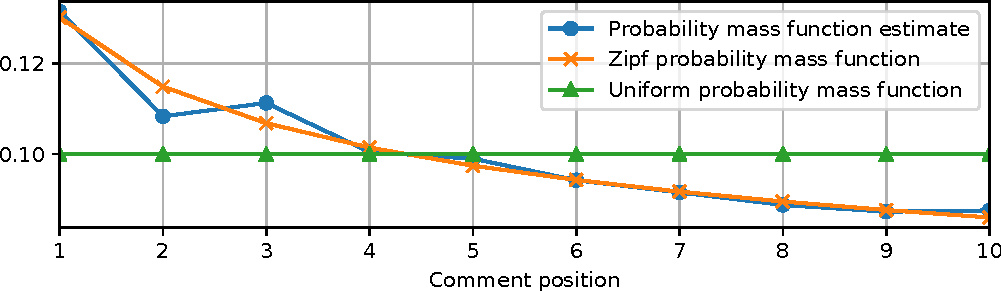
\includegraphics[trim={0cm 0cm 0cm 0cm}, scale=0.75]{figs/quality-evaluation-1}
\caption[Probability mass function estimate $\hat P(\text{at position
}i\mid\text{relevant})$]{%
  Probability mass function (\abbr{pmf}) estimate $\hat
  P(\text{at position }i\mid\text{relevant})$ plotted along the \abbr{pmf} of
  the Zipf distribution with parameters $n=10,$ and $s=0.18$.  If the position
  of a comment and its relevance were independent, we would expect the
  \abbr{pmf} estimate to be uniformly distributed.}
\label{fig:dataset-relevance-analysis}
\end{figure}

To see if this relationship was statistically significant, we modeled the number
of relevant comments at each position~$i$ as a binomial random variable
$X_i\sim \mathrm{Bi}(n, \theta_i)$ with a known number of trials $n=2{,}410$,
and an unknown probability of success $\theta_i$. We then used the one-tailed
Fisher's exact test to reject the following system of null hypotheses at 5\%
significance:
\begin{equation*}
  H_0^{(ij)} : \theta_i = \theta_j,\text{ where }i, j = 1,2,\ldots,10, i < j
\end{equation*}
We rejected $H_0^{(ij)}$ for any $j-i > 3$. Namely, we failed to reject $H_0^{(ij)}$
for $(i,j) = (2,3),$ $(4,5),$ $(5,6),$ $(6,7),$ $(7,8),$ $(7,9),$ $(7,10),$
$(8, 9),$ $(8,10)$, and $(9,10)$. The Benjamini-Hochberg procedure was used to
control the false discovery rate due to multiple testing.

Lastly, we used the subtask~B training dataset to fit a classifier using the
machine learning approach described in Section~\ref{sec:segmentation-result-aggregation}. In
logistic regression, the posterior probability estimate
$\hat P(\textrm{relevant}\mid\mathbf{x}_{uv})$ is modelled as follows:
\begin{equation}
  \ln\frac{\hat P(\textrm{relevant}\mid\mathbf{x}_{uv})}{1-\hat P(\textrm{relevant}\mid
  \mathbf{x}_{uv})}=\beta_0+\bm{\beta}\tran \mathbf{x}_{uv},
\end{equation}
where $\beta_0,\bm{\beta}$\index{.b@$\bm  {\beta }$ (classifier coefficients)|emph} are
the machine-learned coefficients. If we let
$\beta_j,j=1,2,\ldots,24$ denote the individual elements of $\bm{\beta}$\index{.b@$\bm\beta$ (basis)}, then
$|\beta_{i+2}|$, and $|\beta_{i+14}|$ correspond to
the discriminativeness of the elements $m_{1,i+2}$ and $m_{2,i+2}$ in a matrix
$\mathbf{M}_{uv}$\index{.muv@$\mathbf  {M}_{uv}$}. These elements in turn correspond to the score between the
original question text and a comment at position $i$, and the score between the
original question subject and a comment at position $i$ (recall that a thread
consists of twelve nuggets\index{nugget}, which means that $\mathbf{M}_{uv}$ consists of
twelve columns). Plotting $|\beta_{i+2}|$ and $|\beta_{i+14}|$ against the
comment position $i$ in Figure~\ref{fig:segmentation-quality-evaluation-3} shows that
later comments are in general less discriminative than earlier comments. Note
that the classifier discovers this relationship without access to the relevance
judgements about comments.

\begin{figure}[tb]
\centering%
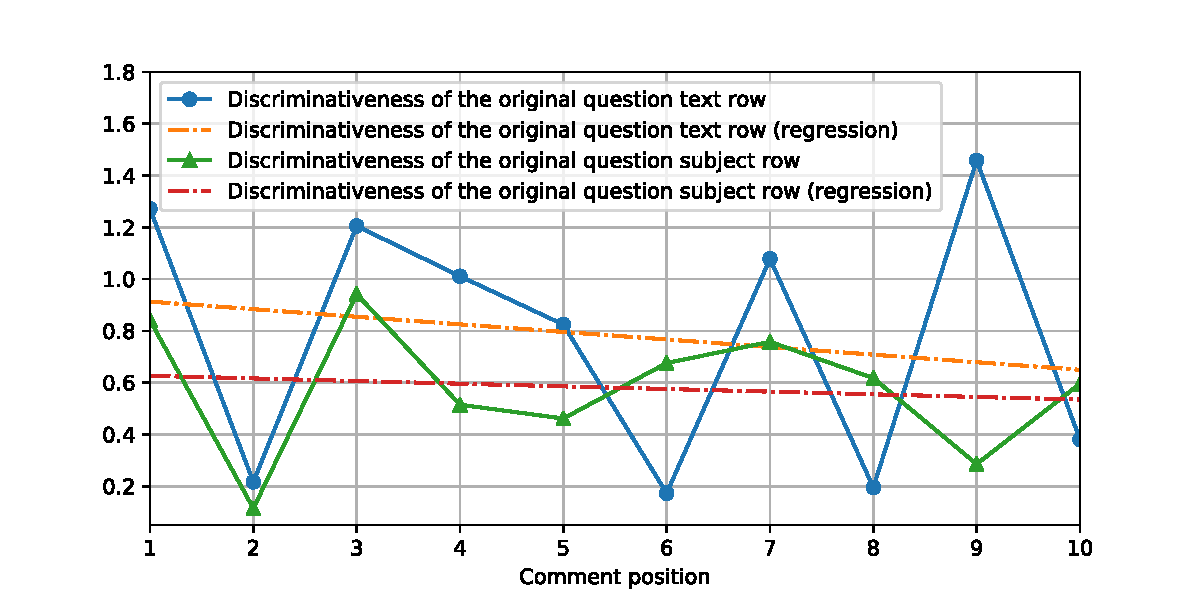
\includegraphics[trim={1.8cm 0.3cm 1.9cm 1.2cm}, scale=0.75]{figs/quality-evaluation-3}
\caption[The discriminativeness of the individual elements of a matrix
$\mathbf{M}_{uv}$ expressed by the absolute values of the machine-learned
coefficients $\bm{\beta}$]{%
  The discriminativeness of the individual elements of a matrix
  $\mathbf{M}_{uv}$\index{.muv@$\mathbf{M}_{uv}$} expressed by the absolute values
  of the machine-learned coefficients $\bm{\beta}$\index{.b@$\bm\beta$ (classifier
  coefficients)}. The discriminativeness of the original question text row
  corresponds to $|\beta_{i+2}|,i=1,2.\ldots,10$, and the discriminativeness of
  the original question subject row corresponds to
  $|\beta_{i+14}|,i=1,2,\ldots,10$.}
  \label{fig:segmentation-quality-evaluation-3}
\end{figure}

These discoveries led us to design and evaluate the
$\wavg_{\textrm{Godwin}}$\index{.wavgGodwin@$\wavg_{\textrm{Godwin}}$|emph}
operator, which assigns a weight proportional to $i^{-1}$ to a nugget\index{nugget} at
position~$i$ in accordance to \term{Zipf's law}\index{Zipf's law}. This
decreases the effect of comments that are likely to be irrelevant. Under the
hypothesis that only relevant comments contain (with a higher chance than
random) important terms that describe the meaning of a document, this weighting
scheme pays attention to scores between those nuggets\index{nugget} that are likely to
contain important terms.

Since weighting terms is conceptually and computationally simpler than
segmentation and result aggregation, we will experimentally verify that the
segmentation is meaningful and that the relevance loss occurs at nugget\index{nugget}
boundaries rather than at term boundaries. For that reason, we designed the
\term{Godwin} term weighting method\index{Godwin!term
weighting|emph}\index{Godwin!operator|see{$\wavg_{\textrm{Godwin}}$}} for the
standard model\index{standard model} scoring function.
For each term $t$ at positions $i_1,i_2,\ldots,i_n$ in a nugget, the method
assigns a weight proportional to $\sum_{j=1}^n i_j^{-1}$ to the
supplementary weight vector element~$e_t$ described in
Section~\ref{sec:segmentation-scoring-function}. It is easy to show that, given
the right choice of term frequency factor (\texttt{t}\index{.t@\texttt{t}} in
Table~\ref{tab:segmentation-smart}) and vector length normalization factor
(\texttt{n}\index{.n@\texttt{n}} in Table~\ref{tab:segmentation-smart}), the
standard model scoring function produces the same ordering on unsegmented
threads as the aggregate scoring function defined in terms of the
$\ominus=\wavg_{\textrm{Godwin}},
\omid=\wavg_{\textrm{length}}$\index{.wavgGodwin@$\wavg_{\textrm{Godwin}}$}
\index{.ominus@$\ominus $}\index{.omid@$\kern .2ex\omid $}
\index{.wavglength@$\wavg _{\textrm  {length}}$} operators would on threads
segmented to one nugget\index{nugget} per a token (see
Figure~\ref{fig:segmentation-weighting}).

\begin{figure}[tb]
\centering
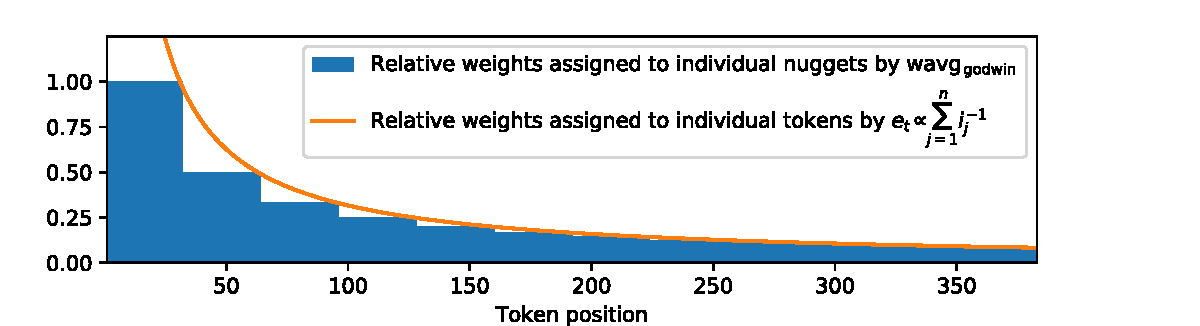
\includegraphics[trim={0.8cm 0.0cm 2.8cm 0.5cm}, scale=0.75]{figs/quality-evaluation-4}
\caption[The relative weights assigned to the individual columns of a matrix
$\mathbf{M}_{uv}$ by the $\wavg_{\textrm{Godwin}}$ operator]{%
  The relative weights assigned to the individual columns of a matrix
  $\mathbf{M}_{uv}$\index{.muv@$\mathbf{M}_{uv}$} by the $\wavg_{\textrm{Godwin}}$ operator plotted along the
  relative weights assigned to the individual tokens by the Godwin term
  weighting\index{Godwin!term weighting} method. The figure assumes the mean
  number of tokens per a thread in the subtask~A unannotated datasets
  (383~tokens), and uniform nugget length in tokens.}
\label{fig:segmentation-weighting}
\end{figure}

\iffalse
\subsubsection{Mutual Information}
\todo{VN: Add the the frequency of 10 terms with the highest ML on the subtask~A
  train dataset in relevant and in the irrelevant comments to conclude that
  there are no terms that can on their discriminate between relevant and
  irrelevant comments. That is why ML is not included in results.}
\fi

\subsection{Parameter estimation}
Some parameters of the scoring functions described in
Section~\ref{sec:segmentation-scoring-function} require careful tuning to each particular
dataset. For the standard model\index{standard model}, this corresponds to the
slope parameter~$s$\index{.s@$s$},
which is used by the normalization factors \texttt{u} and \texttt{b} from
Table~\ref{tab:segmentation-smart} as a part of pivoted document
normalization~\cite{singhaletal95}. For Okapi \abbr{BM}25\index{Okapi
\abbr{BM}25}, this corresponds to the parameters $k_1,k_3,$ and~$b$.%
\index{.k1@$k_1$}\index{.k3@$k_3$}\index{.b@$b$} Apart from
the scoring functions, the parameter~$l$\index{.l@$l$} of the
BestSentence$_l$\index{.bestsentence@BestSentence${}_l$} nugget
filtering method introduced in Section~\ref{sec:segmentation-nugget-filtering}
also requires tuning.

To find the optimum values of $s$\index{.s@$s$}, we initially set $s=0.3$ as
suggested by \textcite{singhaletal95}. By evaluating all the considered
configurations against the subtask~B dev dataset, we obtained the top six
configurations using the normalization factors \texttt{u}\index{.u@\texttt  {u}}
and \texttt{b}\index{.b@\texttt  {b}}, and taking either the unsegmented, machine
learning, or hand-crafted operator approach to result aggregation. We then ran
a grid search to find the values of $s$ in the interval $s\in[0,1]$ maximizing
the performance of these eight configurations.
Figure~\ref{fig:segmentation-slope-optimization} plots the achieved \abbr{MAP}
scores against the choices of parameter~$s$.

\begin{figure}[tb]
\centering%
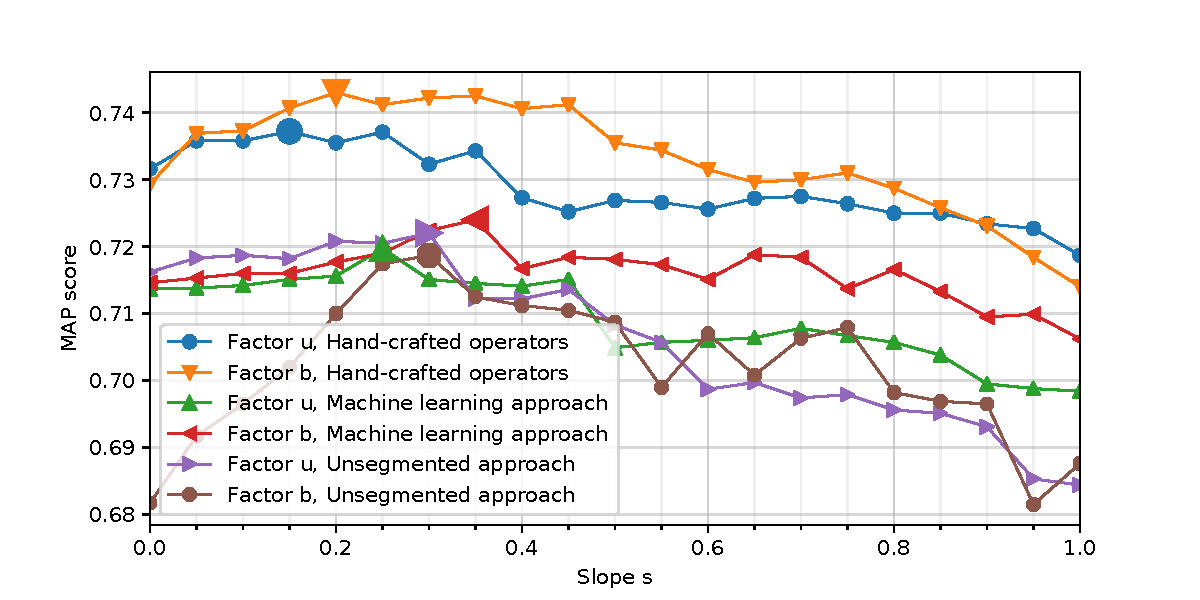
\includegraphics[trim={1.2cm 0.2cm 1.9cm 1.2cm}, scale=0.69]{figs/tfidf}
\caption[The \abbr{MAP} scores achieved with the pivoted normalization factors
\texttt{u} and \texttt{b} for the various choices of the slope parameter~$s$]{%
  The \abbr{MAP} scores achieved with the pivoted normalization factors
  \texttt{u}\index{.u@\texttt{u}} and \texttt{b}\index{.b@\texttt{b}} for the
  various choices of the slope parameter~$s$\index{.s@$s$}.\iffalse Notice that the
  pivoted document normalization is most impactful with the unsegmented
  approach, where the document length varies the most.\fi}
\label{fig:segmentation-slope-optimization}
\end{figure}

To find the optimum values of $k_1,k_3,$ and~$b$\index{.k1@$k_1$}%
\index{.k3@$k_3$}\index{.b@$b$}, we initially set $k_1=1.2,k_3=1000,$
and~$b=0.75$ as suggested by \textcite{singhal01}.
Using the same procedure as above in the intervals $k_1\in[1,2],
k_3\in[0,1000],$ and $b\in[0,1]$, we found the optimal
parameters to be $k_1=2,k_3=950,$ and $b=0$ for the unsegmented approach,
$k_1=2,k_3=0,$ and $b=0.80$ for the machine learning approach, and
$k_1=1.2,k_3=0,$ and $b=0.75$ for the hand-crafted operator approach to result
aggregation.

To find the optimum values of $l$\index{.l@$l$}, we took the
best-performing configuration using the hand-crafted operator approach on the
subtask~B dev dataset (note that
BestSentence$_l$\index{.bestsentence@BestSentence${}_l$} is a nugget
filtering\index{nugget!filtering} method producing a variable number of
nuggets, which makes it unsuitable for both the unsegmented and the machine
learning approach). We then ran a grid search to find the values of $l$ in the
interval $l\in[0,5]$ maximizing the performance of this configuration. Although
\textcite{kolczetal00} suggest the value of $l=3$ in the context of news
articles, the typical question subjects and nuggets\index{nugget} in our
datasets are shorter than the typical news article titles and paragraphs. As a
result, we found more success with less aggressive filtering using $l=0,$ and
$l=1$.

\section{Results}
\label{sec:segmentation-results}
All the 44,496 configurations (twelve~nugget filtering\index{nugget!filtering}
methods, 17~preselected standard model\index{standard model} weighting
schemes, four~supplementary word vectors, four~sets of
Okapi~\abbr{BM}25 parameters\index{Okapi \abbr{BM}25}, 36~pairs of handcrafted
operators, and two~aggregate scoring functions
$S'_{\textrm{query-first}}$ and $S'_{\textrm{result-first}}$) were evaluated on the
\index{.s'queryfirst@$S'_{\text  {query-first}}$}
\index{.s'resultfirst@$S'_{\text  {result-first}}$}
SemEval-2016 and 2017 task~3 subtask~B \abbr{QA} datasets.
Tables~\ref{tab:segmentation-results-2016} and \ref{tab:segmentation-results-2017} show the results.
Although various configurations achieved outstanding \abbr{MAP} scores on one
or the other dataset, only the \term{primary} configuration (highlighted in
bold and italics) consistently achieved scores higher than the winning SemEval
submissions. This configuration uses the \texttt{bfx.nfx} standard model\index{standard model}
weighting scheme suggested by \textcite{ml:SaltonBuckley1988}
for short and homogeneous documents, and the
$\ominus=\wavg_{\textrm{Godwin}}$\index{.wavgGodwin@$\wavg_{\textrm{Godwin}}$}%
\index{.ominus@$\ominus $} handcrafted operator developed in
Section~\ref{sec:segmentation-dataset-analysis}.  This shows that the
$\wavg_{\textrm{Godwin}}$ operator is well-suited to our datasets and hopefully
to \abbr{QA} datasets in general.

Several \term{contrastive} configurations that use the unsegmented approach to
result aggregation were derived from the primary configuration. The contrastive
configuration using the Godwin term weighting\index{Godwin!term weighting}
(denoted \term{\texttt{bfx.nfx}, Godwin} in the tables) performed consistently
worse than the primary configuration, which shows that the segmentation to
nuggets\index{nugget} is meaningful and cannot be replaced with term weighting.

\begin{sidewaystable}[p]
\pagestyle{empty}
\centering
\begin{liningfigs}
\begin{tabular}{lllllll}
Rslt. aggregation &
  Nggt. filtering &
  Scoring function &
  Operator $\ominus$\index{.ominus@$\ominus $} &
  Operator $\omid$\index{.omid@$\kern .2ex\omid $} &
  $S'$\index{.s'@$S'$} &
  \abbr{MAP}\index{map@\abbr {MAP}} \\ \toprule
Handcrafted &
  FirstTwoPara\index{.firsttwopara@FirstTwoPara} &
  \texttt{dpc.ann} &
  $\max$ &
  $\wavg_{\textrm{length}}$\index{.wavglength@$\wavg _{\textrm  {length}}$} &
  $S'_{\textrm{query-first}}$ &
  77.25 \\
Handcrafted &
  --- &
  \texttt{bfx.nfx} &
  $\wavg_{\textrm{Godwin}}$ &
  $\wavg_{\textrm{Godwin}}$ &
  $S'_{\textrm{result-first}}$ &
  \index{.s'resultfirst@$S'_{\text  {result-first}}$}
  77.23 \\
Handcrafted &
  FirstTwoPara &
  \texttt{dpc.ann} &
  $\max$ &
  $\wavg_{\textrm{length}}$ &
  $S'_{\textrm{result-first}}$ &
  77.09 \\
Handcrafted &
  FirstTwoPara &
  \texttt{nfc.dfc}, Murata$_{\textrm B}$\index{.muratab@Murata$_{\textrm B}$} &
  $\avg$ &
  $\min$ &
  $S'_{\textrm{result-first}}$ &
  77.00 \\
Handcrafted &
  FirstTwoPara &
  \texttt{Lpc.ann} &
  $\wavg_{\textrm{length}}$ &
  $\max$ &
  $S'_{\textrm{query-first}}$ &
\index{.s'queryfirst@$S'_{\text  {query-first}}$}
  76.96 \\
\itshape\bfseries Handcrafted &
  --- &
  \bfseries\itshape\texttt{bfx.nfx} &
  \bfseries$\textit{wavg}_{\textit{Godwin}}$\index{.wavgGodwin@$\wavg_{\textrm{Godwin}}$} &
  \bfseries$\textit{wavg}_{\textit{length}}$ &
  \bfseries$\bm S'_{\textit{result-first}}$ &
  \bfseries\itshape76.77 \\
\multicolumn{4}{l}{\bfseries SemEval-2016 task~3 subtask~B winner (\abbr{UH-PRHLT}-primary)} &
  --- &
  --- &
  \bfseries76.70 \\
Unsegmented &
  FirstTwoPara &
  \texttt{Lfb.bfc}, Murata$_{\textrm B}$\index{.muratab@Murata$_{\textrm B}$} &
  --- &
  --- &
  --- &
  76.58 \\
Machine learning &
  FirstPara\index{.firstpara@FirstPara} &
  \texttt{nfc.lfc} &
  --- &
  --- &
  --- &
  75.63 \\
\itshape Unsegmented &
  \itshape FirstTwoPara &
  \itshape\texttt{bfx.nfx} &
  --- &
  --- &
  --- &
  \itshape75.21 \\
\multicolumn{3}{l}{\bfseries SemEval-2016 task~3 subtask~B \abbr{IR}\index{ir@\protect\abbr{IR}} baseline} &
  --- &
  --- &
  --- &
  \bfseries74.75 \\
\itshape Unsegmented &
  --- &
  \itshape\texttt{bfx.nfx} &
  --- &
  --- &
  --- &
  \itshape73.94 \\
\itshape Unsegmented &
  --- &
  \itshape\texttt{bfx.nfx}, Godwin &
  --- &
  --- &
  --- &
  \itshape70.28 \\
\end{tabular}
\end{liningfigs}
\caption[Results for the top five configurations on the 2016
subtask~B test dataset]{%
  Results for the top five configurations on the 2016
  subtask~B test dataset, the primary configuration (highlighted in bold
  and italics) with its contrastive configurations (highlighted in italics),
  the top unsegmented and machine learning configurations. The
  \abbr{IR} baseline and the winning submission are highlighted in
  bold.}
\label{tab:segmentation-results-2016}
\end{sidewaystable}

\begin{sidewaystable}[p]
\centering
\begin{liningfigs}
\begin{tabular}{lllllll}
Rslt. aggregation &
  Nggt. filtering &
  Scoring function &
  Operator $\ominus$\index{.ominus@$\ominus $} &
  Operator $\omid$\index{.omid@$\kern .2ex\omid $} &
  $S'$\index{.s'@$S'$} &
  \abbr{MAP}\index{map@\abbr {MAP}} \\ \toprule
Handcrafted &
  BestSentence$_0$\index{.bestsentence@BestSentence${}_l$} &
  Okapi \abbr{BM}25 &
  $\avg$ &
  $\max$ &
  $S'_{\textrm{result-first}}$ &
  49.20 \\
Handcrafted &
  BestSentence$_0$ &
  Okapi \abbr{BM}25 &
  $\avg$ &
  $\wavg_{\textrm{Godwin}}$\index{.wavgGodwin@$\wavg_{\textrm{Godwin}}$} &
  $S'_{\textrm{result-first}}$ &
  \index{.s'resultfirst@$S'_{\text  {result-first}}$}
  48.87 \\
Handcrafted &
  BestSentence$_0$ &
  Okapi \abbr{BM}25 &
  $\avg$ &
  $\max$ &
  $S'_{\textrm{query-first}}$ &
  \index{.s'queryfirst@$S'_{\text  {query-first}}$}
  48.79 \\
Handcrafted &
  BestSentence$_0$ &
  \texttt{bfx.nfx}, Murata$_{\textrm A}$\index{.murataa@Murata$_{\textrm A}$} &
  $\max$ &
  $\wavg_{\textrm{Godwin}}$ &
  $S'_{\textrm{result-first}}$ &
  48.76 \\
Handcrafted &
  BestSentence$_0$ &
  Okapi \abbr{BM}25 &
  $\avg$ &
  $\wavg_{\textrm{Godwin}}$ &
  $S'_{\textrm{result-first}}$ &
  48.76 \\
Unsegmented &
  FirstTwoPara\index{.firsttwopara@FirstTwoPara} &
  \texttt{Lpu.Lpc}, Murata$_{\textrm A}$\index{.murataa@Murata$_{\textrm A}$} &
  --- &
  --- &
  --- &
  48.75 \\
\bfseries\itshape Handcrafted &
  --- &
  \bfseries\itshape\texttt{bfx.nfx} &
  \bfseries$\textit{wavg}_{\textit{Godwin}}$ &
  \bfseries$\textit{wavg}_{\textit{length}}$ &
  \bfseries$\bm S'_{\textit{result-first}}$ &
  \bfseries\itshape47.45 \\
\multicolumn{4}{l}{\bfseries SemEval-2017 task~3 subtask~B winner (SimBow-primary)} &
  --- &
  --- &
  \bfseries47.22 \\
Machine learning &
  FirstTwoPara &
  \texttt{bfx.nfx} &
  --- &
  --- &
  --- &
  46.90 \\
\itshape Unsegmented &
  \itshape FirstTwoPara &
  \itshape\texttt{bfx.nfx} &
  --- &
  --- &
  --- &
  \itshape44.67 \\
\multicolumn{3}{l}{\bfseries SemEval-2017 task~3 subtask~B \abbr{IR}\index{ir@\protect\abbr{IR}} baseline} &
  --- &
  --- &
  --- &
  \bfseries41.85 \\
\itshape Unsegmented &
  --- &
  \itshape\texttt{bfx.nfx}, Godwin &
  --- &
  --- &
  --- &
  \itshape37.18 \\
  %this is baseline, right? any way to tell it to the reader?
\itshape Unsegmented &
  --- &
  \itshape\texttt{bfx.nfx} &
  --- &
  --- &
  --- &
  \itshape36.82 \\
\end{tabular}
\end{liningfigs}
\caption[Results for the top five configurations on the 2017
subtask~B test dataset]{%
  Results for the top five configurations on the 2017
  subtask~B test dataset, the primary configuration (highlighted in bold
  and italics) with its contrastive configurations (highlighted in italics),
  the top unsegmented and machine learning configurations. The
  \abbr{IR} baseline and the winning submission are highlighted in
  bold.}
\label{tab:segmentation-results-2017}
\end{sidewaystable}

The two remaining contrastive configurations using no nugget filtering and the
FirstTwoPara\index{.firsttwopara@FirstTwoPara} nugget
filtering\index{nugget!filtering} show that without segmentation, the standard
model\index{standard model} is unable to cope with the outlier terms introduced by irrelevant
comments. Removing all nuggets\index{nugget} other than the question subject and text
improves the \abbr{MAP} score, but at the cost of losing important terms. The
primary configuration achieves the highest \abbr{MAP} score by properly
weighting the individual nuggets\index{nugget}.

\iffalse
\todo{VN: Significance tests a Density of MAP figures, see:
  \url{https://km.aifb.kit.edu/ws/semsearch10/Files/bm25f.pdf\#page=7}}

\subsubsection{Qualitative Analysis}
\label{sec:segmentation-qualitative-analysis}
\todo{VN: %
  \url{https://gitlab.fi.muni.cz/xnovot32/segmentation-experiments/blob/old-quality-evaluation/quality\_evaluation/quality\_evaluation.ipynb},
  although it would be ideal to update the code as well as the tested configuration
  before publishing.}
\fi

\section{Conclusion and future work}
\label{sec:segmentation-conclusion}
Segmentation matters and so does careful weighting. By combining both, we were
able to achieve state-of-the-art results on the SemEval-2016 and 2017 task~3
subtask~B \abbr{QA} datasets using the standard bag-of-words vector space
model\index{standard model} without semantic modelling. Our method can be
readily implemented into existing inverted-index-based search engines.

\ifreview
Rygl\etal~\cite{rygletal17} have recently shown
\else
We have recently shown~\cite{rygletal17}
\fi
that arbitrary vector space models (e.g.\ \abbr{LSA}\index{LSA@\abbr{LSA}},
\abbr{LDA}, Doc2vec\index{Doc2vec}, \ldots\kern-.2ex) can be used to represent documents
in inverted-index-based search engines.
Evaluating how the concepts of segmentation and result aggregation interact
with semantic models that are not based on a bag-of-words representation
is an intriguing direction for future research.

We have shown \ifthesis in Section~\ref{sec:segmentation-dataset-analysis} \fi that there is a
statistically significant relationship between the position of a comment and
its relevance in the SemEval-2016 and 2017 subtask~A datasets. Investigating whether such a relationship exists in other \abbr{QA} datasets (and other datasets in
general) will provide us with new insights to the dynamics of online discourse and
lead to more effective retrieval systems.

\iffalse
As shown in Section~\ref{sec:segmentation-dataset-analysis}, there is a statistically
significant relationship between the position of a comment and its relevance
in the SemEval-2016 and 2017 subtask~A datasets. This may 
\todo{VN: Segmentation does matter, but depends on data (Godwin weighting for QA
dataset).  Good term weighting does matter, too.  Taking care of both, we gain
best results on Semeval data even with the standard bag-of-words vector space
representations.}
\todo{VN: We have recently shown how arbitrary vector-space models, such as the
  bag-of-topics LSA and LDA vector spaces, can be represented in
  inverted-index-based search engines:
  \url{http://www.aclweb.org/anthology/W17-2611} How would our system work
  on general vector space models?}
\todo{VN: Would the detection of phrases help our model? Initial testing suggests
  that it would not:
  \url{https://gitlab.fi.muni.cz/xnovot32/segmentation-experiments/wikis/report-2017-10-11}
  but we did not do detection on sequences to filter out incorrectly-detected
  phrases and neither did we try to include both the original phrase and its
  constituents into the document vector. (Perhaps show a table of the top-ranking
  phrase candidates.)}
\todo{VN: How well do our methods generalize to other datasets?}
\todo{VN: The machine learning segmented approach can be generalized to
  documents with a variable number of nuggets by normalizing the dimensions of
  the pairwise nugget similarity matrix, or by treating the matrix as an image
  and the relevance prediction problem as an image classification problem. No
  experiments were conducted to test the performance of this model.}
\todo{VN: How well do our methods generalize to other datasets?}
\todo{VN: (Kołcz\etal 2000, sec. 4) suggests the use of mutual information for term weighting when classification data is available}
\fi

\ifreview\else
\subsection*{Acknowledgments}
\abbr{\noexpand\MakeUppercase TAČR} Omega grant \abbr{TD03000295} is gratefully acknowledged.
\fi

%% The following section corresponds to the bibliography:
\nocite{ir:Zezula2006} %% The recommended literature.
\nocite{ml:IntroIR2008}
\nocite{mikolov2013efficient}
\begingroup\sloppy
\printbibliography[heading=bibintoc]
\endgroup

\end{document}
